%--------------------------------------
%ELECTROTECHNIQUE - SCHEMA DE LIAISON A LA TERRE
%--------------------------------------

%utiliser les environnement \begin{comment} \end{comment} pour mettre en commentaire le préambule une fois la programmation appelée dans le document maître (!ne pas oublier de mettre en commentaire \end{document}!)

\begin{comment}

\documentclass[a4paper, 11pt, twoside, fleqn]{memoir}

\usepackage{AOCDTF}

\marqueurchapitre

%lien de l'éditeur : https://www.mathcha.io/editor/W9VrNux1SnLu4o3Jm4hklNKwvuOwJ7XwCV6yqOW

%--------------------------------------
%corps du document
%--------------------------------------

\begin{document} %corps du document
	\openleft %début de chapitre à gauche

\end{comment}

\begin{figure}[H]
\caption{Boucle de défaut du courant $I_d$ sur L1}




\tikzset{every picture/.style={line width=0.75pt}} %set default line width to 0.75pt        

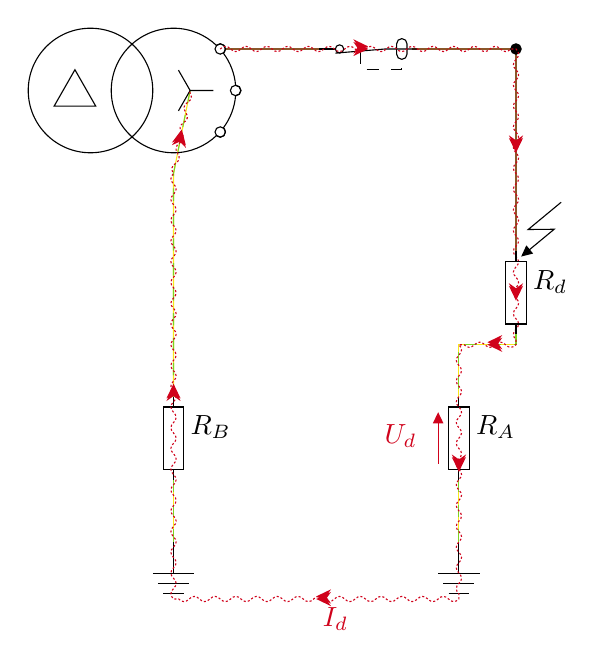
\begin{tikzpicture}[x=0.75pt,y=0.75pt,yscale=-1,xscale=1]
%uncomment if require: \path (0,353); %set diagram left start at 0, and has height of 353

%Straight Lines [id:da8450582290113836] 
\draw [color={rgb, 255:red, 248; green, 231; blue, 28 }  ,draw opacity=1 ]   (87.5,222.5) -- (87.5,252.5) ;
%Straight Lines [id:da035234150750507176] 
\draw [color={rgb, 255:red, 248; green, 231; blue, 28 }  ,draw opacity=1 ]   (252.5,152.5) -- (252.5,157.5) -- (225,157.5) -- (225,182.5) ;
%Straight Lines [id:da575921985906619] 
\draw [color={rgb, 255:red, 139; green, 87; blue, 42 }  ,draw opacity=1 ]   (112.5,15) -- (162.5,15) ;
%Straight Lines [id:da5726536295563455] 
\draw [color={rgb, 255:red, 248; green, 231; blue, 28 }  ,draw opacity=1 ]   (95.5,35) -- (87.5,75) -- (87.5,182.5) ;
%Straight Lines [id:da38476257001275427] 
\draw [color={rgb, 255:red, 126; green, 211; blue, 33 }  ,draw opacity=1 ] [dash pattern={on 4.5pt off 4.5pt}]  (95.5,35) -- (87.5,75) -- (87.5,182.5) ;
%Straight Lines [id:da9973940303994429] 
\draw [color={rgb, 255:red, 139; green, 87; blue, 42 }  ,draw opacity=1 ]   (202.5,15) -- (252.5,15) ;
%Shape: Path Data [id:dp9822778342813306] 
\draw   (112.5,55) .. controls (112.5,56.38) and (111.38,57.5) .. (110,57.5) .. controls (109.29,57.5) and (108.65,57.2) .. (108.19,56.72) .. controls (102.81,61.85) and (95.52,65) .. (87.5,65) .. controls (70.93,65) and (57.5,51.57) .. (57.5,35) .. controls (57.5,18.43) and (70.93,5) .. (87.5,5) .. controls (95.52,5) and (102.81,8.15) .. (108.19,13.28) .. controls (108.65,12.8) and (109.29,12.5) .. (110,12.5) .. controls (111.38,12.5) and (112.5,13.62) .. (112.5,15) .. controls (112.5,15.82) and (112.11,16.54) .. (111.5,17) .. controls (114.8,21.39) and (116.92,26.71) .. (117.4,32.5) .. controls (117.43,32.5) and (117.47,32.5) .. (117.5,32.5) .. controls (118.88,32.5) and (120,33.62) .. (120,35) .. controls (120,36.38) and (118.88,37.5) .. (117.5,37.5) .. controls (117.47,37.5) and (117.43,37.5) .. (117.4,37.5) .. controls (116.92,43.29) and (114.8,48.61) .. (111.5,53) .. controls (112.11,53.46) and (112.5,54.18) .. (112.5,55) -- cycle ;
%Shape: Circle [id:dp10169246549820965] 
\draw   (17.5,35) .. controls (17.5,18.43) and (30.93,5) .. (47.5,5) .. controls (64.07,5) and (77.5,18.43) .. (77.5,35) .. controls (77.5,51.57) and (64.07,65) .. (47.5,65) .. controls (30.93,65) and (17.5,51.57) .. (17.5,35) -- cycle ;
%Shape: Triangle [id:dp22185224755779764] 
\draw   (40,25) -- (30,42.5) -- (50,42.5) -- cycle ;
%Shape: Star [id:dp4535075510124722] 
\draw   (106.75,35) -- (95.5,35) -- (89.88,44.81) -- (95.5,35) -- (89.88,25.19) -- (95.5,35) -- cycle ;
%Shape: Circle [id:dp28187455970704567] 
\draw   (107.5,15) .. controls (107.5,13.62) and (108.62,12.5) .. (110,12.5) .. controls (111.38,12.5) and (112.5,13.62) .. (112.5,15) .. controls (112.5,16.38) and (111.38,17.5) .. (110,17.5) .. controls (108.62,17.5) and (107.5,16.38) .. (107.5,15) -- cycle ;
%Shape: Circle [id:dp9096244123377861] 
\draw   (114.9,35) .. controls (114.9,33.62) and (116.02,32.5) .. (117.4,32.5) .. controls (118.78,32.5) and (119.9,33.62) .. (119.9,35) .. controls (119.9,36.38) and (118.78,37.5) .. (117.4,37.5) .. controls (116.02,37.5) and (114.9,36.38) .. (114.9,35) -- cycle ;
%Shape: Circle [id:dp0660770114066822] 
\draw   (107.5,55) .. controls (107.5,53.62) and (108.62,52.5) .. (110,52.5) .. controls (111.38,52.5) and (112.5,53.62) .. (112.5,55) .. controls (112.5,56.38) and (111.38,57.5) .. (110,57.5) .. controls (108.62,57.5) and (107.5,56.38) .. (107.5,55) -- cycle ;

%Straight Lines [id:da12486709959480935] 
\draw [color={rgb, 255:red, 139; green, 87; blue, 42 }  ,draw opacity=1 ]   (252.5,112.5) -- (252.5,17.5) ;
%Straight Lines [id:da9194886303106931] 
\draw [color={rgb, 255:red, 126; green, 211; blue, 33 }  ,draw opacity=1 ] [dash pattern={on 4.5pt off 4.5pt}]  (252.5,152.5) -- (252.5,157.5) -- (225,157.5) -- (225,182.5) ;
%Straight Lines [id:da33889517147418446] 
\draw    (87.5,252.5) -- (87.5,267.5) ;
%Straight Lines [id:da7536356147270271] 
\draw    (77.5,267.5) -- (97.5,267.5) ;
%Straight Lines [id:da33790733335159795] 
\draw    (80,272.5) -- (95,272.5) ;
%Straight Lines [id:da8225336413065082] 
\draw    (82.5,277.5) -- (92.5,277.5) ;

%Straight Lines [id:da14728368722832463] 
\draw [color={rgb, 255:red, 126; green, 211; blue, 33 }  ,draw opacity=1 ] [dash pattern={on 4.5pt off 4.5pt}]  (87.5,222.5) -- (87.5,252.5) ;
%Straight Lines [id:da2713756434582886] 
\draw [color={rgb, 255:red, 248; green, 231; blue, 28 }  ,draw opacity=1 ]   (225,222.5) -- (225,252.5) ;
%Straight Lines [id:da07200185094723521] 
\draw    (225,252.5) -- (225,267.5) ;
%Straight Lines [id:da5503731135148442] 
\draw    (215,267.5) -- (235,267.5) ;
%Straight Lines [id:da9244125108161202] 
\draw    (217.5,272.5) -- (232.5,272.5) ;
%Straight Lines [id:da07512791048030887] 
\draw    (220,277.5) -- (230,277.5) ;

%Straight Lines [id:da5491926071123034] 
\draw [color={rgb, 255:red, 126; green, 211; blue, 33 }  ,draw opacity=1 ] [dash pattern={on 4.5pt off 4.5pt}]  (225,222.5) -- (225,252.5) ;
%Straight Lines [id:da7705666086878261] 
\draw    (87.5,217.5) -- (87.5,222.5) ;
%Shape: Rectangle [id:dp5724900932521552] 
\draw   (92.5,187.5) -- (92.5,217.5) -- (82.5,217.5) -- (82.5,187.5) -- cycle ;
%Straight Lines [id:da6857493814799358] 
\draw    (87.5,182.5) -- (87.5,187.5) ;

%Straight Lines [id:da7810225170823131] 
\draw    (225,217.5) -- (225,222.5) ;
%Shape: Rectangle [id:dp9839408028922504] 
\draw   (230,187.5) -- (230,217.5) -- (220,217.5) -- (220,187.5) -- cycle ;
%Straight Lines [id:da4367313473487816] 
\draw    (225,182.5) -- (225,187.5) ;

%Shape: Circle [id:dp6401617010113628] 
\draw  [fill={rgb, 255:red, 0; green, 0; blue, 0 }  ,fill opacity=1 ] (250,15) .. controls (250,13.62) and (251.12,12.5) .. (252.5,12.5) .. controls (253.88,12.5) and (255,13.62) .. (255,15) .. controls (255,16.38) and (253.88,17.5) .. (252.5,17.5) .. controls (251.12,17.5) and (250,16.38) .. (250,15) -- cycle ;
%Rounded Rect [id:dp9837999595449706] 
\draw   (197.5,20) .. controls (196.12,20) and (195,18.88) .. (195,17.5) -- (195,12.5) .. controls (195,11.12) and (196.12,10) .. (197.5,10) -- (197.5,10) .. controls (198.88,10) and (200,11.12) .. (200,12.5) -- (200,17.5) .. controls (200,18.88) and (198.88,20) .. (197.5,20) -- cycle ;
%Straight Lines [id:da04140906911364939] 
\draw  [dash pattern={on 4.5pt off 4.5pt}]  (177.5,16) -- (177.5,25) -- (197.5,25) -- (197.5,20) ;
%Shape: Circle [id:dp7012058816599942] 
\draw   (167.5,13) .. controls (166.4,13) and (165.5,13.9) .. (165.5,15) .. controls (165.5,16.1) and (166.4,17) .. (167.5,17) .. controls (168.6,17) and (169.5,16.1) .. (169.5,15) .. controls (169.5,13.9) and (168.6,13) .. (167.5,13) -- cycle ;
%Straight Lines [id:da23692932983683102] 
\draw    (165.5,15) -- (157.5,15) ;
%Straight Lines [id:da4567235518407359] 
\draw    (165.5,17) -- (189.5,15) -- (205,15) ;
%Shape: Boxed Line [id:dp44753967705251496] 
\draw    (274.27,88.83) -- (258.39,101.97) -- (270.89,101.86) -- (257.31,113.09) ;
\draw [shift={(255,115)}, rotate = 320.40999999999997] [fill={rgb, 255:red, 0; green, 0; blue, 0 }  ][line width=0.08]  [draw opacity=0] (5.36,-2.57) -- (0,0) -- (5.36,2.57) -- cycle    ;
\draw [color={rgb, 255:red, 208; green, 2; blue, 27 }  ,draw opacity=1 ] [dash pattern={on 0.75pt off 0.75pt}]  (110,15) .. controls (111.67,13.33) and (113.33,13.33) .. (115,15) .. controls (116.67,16.67) and (118.33,16.67) .. (120,15) .. controls (121.67,13.33) and (123.33,13.33) .. (125,15) .. controls (126.67,16.67) and (128.33,16.67) .. (130,15) .. controls (131.67,13.33) and (133.33,13.33) .. (135,15) .. controls (136.67,16.67) and (138.33,16.67) .. (140,15) .. controls (141.67,13.33) and (143.33,13.33) .. (145,15) .. controls (146.67,16.67) and (148.33,16.67) .. (150,15) .. controls (151.67,13.33) and (153.33,13.33) .. (155,15) .. controls (156.67,16.67) and (158.33,16.67) .. (160,15) .. controls (161.67,13.33) and (163.33,13.33) .. (165,15) .. controls (166.67,16.67) and (168.33,16.67) .. (170,15) .. controls (171.67,13.33) and (173.33,13.33) .. (175,15) .. controls (176.67,16.67) and (178.33,16.67) .. (180,15) .. controls (181.67,13.33) and (183.33,13.33) .. (185,15) .. controls (186.67,16.67) and (188.33,16.67) .. (190,15) .. controls (191.67,13.33) and (193.33,13.33) .. (195,15) .. controls (196.67,16.67) and (198.33,16.67) .. (200,15) .. controls (201.67,13.33) and (203.33,13.33) .. (205,15) .. controls (206.67,16.67) and (208.33,16.67) .. (210,15) .. controls (211.67,13.33) and (213.33,13.33) .. (215,15) .. controls (216.67,16.67) and (218.33,16.67) .. (220,15) .. controls (221.67,13.33) and (223.33,13.33) .. (225,15) .. controls (226.67,16.67) and (228.33,16.67) .. (230,15) .. controls (231.67,13.33) and (233.33,13.33) .. (235,15) .. controls (236.67,16.67) and (238.33,16.67) .. (240,15) .. controls (241.67,13.33) and (243.33,13.33) .. (245,15) .. controls (246.67,16.67) and (248.33,16.67) .. (250,15) -- (252.5,15) -- (252.5,15) .. controls (254.17,16.67) and (254.17,18.33) .. (252.5,20) .. controls (250.83,21.67) and (250.83,23.33) .. (252.5,25) .. controls (254.17,26.67) and (254.17,28.33) .. (252.5,30) .. controls (250.83,31.67) and (250.83,33.33) .. (252.5,35) .. controls (254.17,36.67) and (254.17,38.33) .. (252.5,40) .. controls (250.83,41.67) and (250.83,43.33) .. (252.5,45) .. controls (254.17,46.67) and (254.17,48.33) .. (252.5,50) .. controls (250.83,51.67) and (250.83,53.33) .. (252.5,55) .. controls (254.17,56.67) and (254.17,58.33) .. (252.5,60) .. controls (250.83,61.67) and (250.83,63.33) .. (252.5,65) .. controls (254.17,66.67) and (254.17,68.33) .. (252.5,70) .. controls (250.83,71.67) and (250.83,73.33) .. (252.5,75) .. controls (254.17,76.67) and (254.17,78.33) .. (252.5,80) .. controls (250.83,81.67) and (250.83,83.33) .. (252.5,85) .. controls (254.17,86.67) and (254.17,88.33) .. (252.5,90) .. controls (250.83,91.67) and (250.83,93.33) .. (252.5,95) .. controls (254.17,96.67) and (254.17,98.33) .. (252.5,100) .. controls (250.83,101.67) and (250.83,103.33) .. (252.5,105) .. controls (254.17,106.67) and (254.17,108.33) .. (252.5,110) .. controls (250.83,111.67) and (250.83,113.33) .. (252.5,115) -- (252.5,115) .. controls (254.17,116.67) and (254.17,118.33) .. (252.5,120) .. controls (250.83,121.67) and (250.83,123.33) .. (252.5,125) .. controls (254.17,126.67) and (254.17,128.33) .. (252.5,130) .. controls (250.83,131.67) and (250.83,133.33) .. (252.5,135) .. controls (254.17,136.67) and (254.17,138.33) .. (252.5,140) .. controls (250.83,141.67) and (250.83,143.33) .. (252.5,145) .. controls (254.17,146.67) and (254.17,148.33) .. (252.5,150) .. controls (250.83,151.67) and (250.83,153.33) .. (252.5,155) -- (252.5,157.5) -- (252.5,157.5) .. controls (250.83,159.17) and (249.17,159.17) .. (247.5,157.5) .. controls (245.83,155.83) and (244.17,155.83) .. (242.5,157.5) .. controls (240.83,159.17) and (239.17,159.17) .. (237.5,157.5) .. controls (235.83,155.83) and (234.17,155.83) .. (232.5,157.5) .. controls (230.83,159.17) and (229.17,159.17) .. (227.5,157.5) -- (225,157.5) -- (225,157.5) .. controls (226.67,159.17) and (226.67,160.83) .. (225,162.5) .. controls (223.33,164.17) and (223.33,165.83) .. (225,167.5) .. controls (226.67,169.17) and (226.67,170.83) .. (225,172.5) .. controls (223.33,174.17) and (223.33,175.83) .. (225,177.5) .. controls (226.67,179.17) and (226.67,180.83) .. (225,182.5) .. controls (223.33,184.17) and (223.33,185.83) .. (225,187.5) .. controls (226.67,189.17) and (226.67,190.83) .. (225,192.5) .. controls (223.33,194.17) and (223.33,195.83) .. (225,197.5) .. controls (226.67,199.17) and (226.67,200.83) .. (225,202.5) .. controls (223.33,204.17) and (223.33,205.83) .. (225,207.5) .. controls (226.67,209.17) and (226.67,210.83) .. (225,212.5) .. controls (223.33,214.17) and (223.33,215.83) .. (225,217.5) .. controls (226.67,219.17) and (226.67,220.83) .. (225,222.5) .. controls (223.33,224.17) and (223.33,225.83) .. (225,227.5) .. controls (226.67,229.17) and (226.67,230.83) .. (225,232.5) .. controls (223.33,234.17) and (223.33,235.83) .. (225,237.5) .. controls (226.67,239.17) and (226.67,240.83) .. (225,242.5) .. controls (223.33,244.17) and (223.33,245.83) .. (225,247.5) .. controls (226.67,249.17) and (226.67,250.83) .. (225,252.5) .. controls (223.33,254.17) and (223.33,255.83) .. (225,257.5) .. controls (226.67,259.17) and (226.67,260.83) .. (225,262.5) .. controls (223.33,264.17) and (223.33,265.83) .. (225,267.5) .. controls (226.67,269.17) and (226.67,270.83) .. (225,272.5) .. controls (223.33,274.17) and (223.33,275.83) .. (225,277.5) -- (225,280) -- (225,280) .. controls (223.33,281.67) and (221.67,281.67) .. (220,280) .. controls (218.33,278.33) and (216.67,278.33) .. (215,280) .. controls (213.33,281.67) and (211.67,281.67) .. (210,280) .. controls (208.33,278.33) and (206.67,278.33) .. (205,280) .. controls (203.33,281.67) and (201.67,281.67) .. (200,280) .. controls (198.33,278.33) and (196.67,278.33) .. (195,280) .. controls (193.33,281.67) and (191.67,281.67) .. (190,280) .. controls (188.33,278.33) and (186.67,278.33) .. (185,280) .. controls (183.33,281.67) and (181.67,281.67) .. (180,280) .. controls (178.33,278.33) and (176.67,278.33) .. (175,280) .. controls (173.33,281.67) and (171.67,281.67) .. (170,280) .. controls (168.33,278.33) and (166.67,278.33) .. (165,280) .. controls (163.33,281.67) and (161.67,281.67) .. (160,280) .. controls (158.33,278.33) and (156.67,278.33) .. (155,280) .. controls (153.33,281.67) and (151.67,281.67) .. (150,280) .. controls (148.33,278.33) and (146.67,278.33) .. (145,280) .. controls (143.33,281.67) and (141.67,281.67) .. (140,280) .. controls (138.33,278.33) and (136.67,278.33) .. (135,280) .. controls (133.33,281.67) and (131.67,281.67) .. (130,280) .. controls (128.33,278.33) and (126.67,278.33) .. (125,280) .. controls (123.33,281.67) and (121.67,281.67) .. (120,280) .. controls (118.33,278.33) and (116.67,278.33) .. (115,280) .. controls (113.33,281.67) and (111.67,281.67) .. (110,280) .. controls (108.33,278.33) and (106.67,278.33) .. (105,280) .. controls (103.33,281.67) and (101.67,281.67) .. (100,280) .. controls (98.33,278.33) and (96.67,278.33) .. (95,280) .. controls (93.33,281.67) and (91.67,281.67) .. (90,280) -- (87.5,280) -- (87.5,280) .. controls (85.83,278.33) and (85.83,276.67) .. (87.5,275) .. controls (89.17,273.33) and (89.17,271.67) .. (87.5,270) .. controls (85.83,268.33) and (85.83,266.67) .. (87.5,265) .. controls (89.17,263.33) and (89.17,261.67) .. (87.5,260) .. controls (85.83,258.33) and (85.83,256.67) .. (87.5,255) .. controls (89.17,253.33) and (89.17,251.67) .. (87.5,250) .. controls (85.83,248.33) and (85.83,246.67) .. (87.5,245) .. controls (89.17,243.33) and (89.17,241.67) .. (87.5,240) .. controls (85.83,238.33) and (85.83,236.67) .. (87.5,235) .. controls (89.17,233.33) and (89.17,231.67) .. (87.5,230) .. controls (85.83,228.33) and (85.83,226.67) .. (87.5,225) .. controls (89.17,223.33) and (89.17,221.67) .. (87.5,220) .. controls (85.83,218.33) and (85.83,216.67) .. (87.5,215) .. controls (89.17,213.33) and (89.17,211.67) .. (87.5,210) .. controls (85.83,208.33) and (85.83,206.67) .. (87.5,205) .. controls (89.17,203.33) and (89.17,201.67) .. (87.5,200) .. controls (85.83,198.33) and (85.83,196.67) .. (87.5,195) .. controls (89.17,193.33) and (89.17,191.67) .. (87.5,190) .. controls (85.83,188.33) and (85.83,186.67) .. (87.5,185) .. controls (89.17,183.33) and (89.17,181.67) .. (87.5,180) .. controls (85.83,178.33) and (85.83,176.67) .. (87.5,175) .. controls (89.17,173.33) and (89.17,171.67) .. (87.5,170) .. controls (85.83,168.33) and (85.83,166.67) .. (87.5,165) .. controls (89.17,163.33) and (89.17,161.67) .. (87.5,160) .. controls (85.83,158.33) and (85.83,156.67) .. (87.5,155) .. controls (89.17,153.33) and (89.17,151.67) .. (87.5,150) .. controls (85.83,148.33) and (85.83,146.67) .. (87.5,145) .. controls (89.17,143.33) and (89.17,141.67) .. (87.5,140) .. controls (85.83,138.33) and (85.83,136.67) .. (87.5,135) .. controls (89.17,133.33) and (89.17,131.67) .. (87.5,130) .. controls (85.83,128.33) and (85.83,126.67) .. (87.5,125) .. controls (89.17,123.33) and (89.17,121.67) .. (87.5,120) .. controls (85.83,118.33) and (85.83,116.67) .. (87.5,115) .. controls (89.17,113.33) and (89.17,111.67) .. (87.5,110) .. controls (85.83,108.33) and (85.83,106.67) .. (87.5,105) .. controls (89.17,103.33) and (89.17,101.67) .. (87.5,100) .. controls (85.83,98.33) and (85.83,96.67) .. (87.5,95) .. controls (89.17,93.33) and (89.17,91.67) .. (87.5,90) .. controls (85.83,88.33) and (85.83,86.67) .. (87.5,85) .. controls (89.17,83.33) and (89.17,81.67) .. (87.5,80) .. controls (85.83,78.33) and (85.83,76.67) .. (87.5,75) -- (87.5,75) .. controls (86.19,73.04) and (86.52,71.41) .. (88.48,70.1) .. controls (90.44,68.79) and (90.77,67.15) .. (89.46,65.19) .. controls (88.15,63.23) and (88.48,61.6) .. (90.44,60.29) .. controls (92.4,58.98) and (92.73,57.35) .. (91.42,55.39) .. controls (90.11,53.43) and (90.44,51.8) .. (92.4,50.49) .. controls (94.36,49.18) and (94.69,47.54) .. (93.38,45.58) .. controls (92.07,43.62) and (92.4,41.99) .. (94.36,40.68) .. controls (96.32,39.37) and (96.65,37.74) .. (95.34,35.78) -- (95.5,35) -- (95.5,35) ;
\draw [shift={(181.25,15)}, rotate = 180] [fill={rgb, 255:red, 208; green, 2; blue, 27 }  ,fill opacity=1 ][line width=0.08]  [draw opacity=0] (7.14,-3.43) -- (0,0) -- (7.14,3.43) -- (4.74,0) -- cycle    ;
\draw [shift={(252.5,65)}, rotate = 270] [fill={rgb, 255:red, 208; green, 2; blue, 27 }  ,fill opacity=1 ][line width=0.08]  [draw opacity=0] (7.14,-3.43) -- (0,0) -- (7.14,3.43) -- (4.74,0) -- cycle    ;
\draw [shift={(252.5,136.25)}, rotate = 270] [fill={rgb, 255:red, 208; green, 2; blue, 27 }  ,fill opacity=1 ][line width=0.08]  [draw opacity=0] (7.14,-3.43) -- (0,0) -- (7.14,3.43) -- (4.74,0) -- cycle    ;
\draw [shift={(238.75,157.5)}, rotate = 360] [fill={rgb, 255:red, 208; green, 2; blue, 27 }  ,fill opacity=1 ][line width=0.08]  [draw opacity=0] (7.14,-3.43) -- (0,0) -- (7.14,3.43) -- (4.74,0) -- cycle    ;
\draw [shift={(225,218.75)}, rotate = 270] [fill={rgb, 255:red, 208; green, 2; blue, 27 }  ,fill opacity=1 ][line width=0.08]  [draw opacity=0] (7.14,-3.43) -- (0,0) -- (7.14,3.43) -- (4.74,0) -- cycle    ;
\draw [shift={(156.25,280)}, rotate = 360] [fill={rgb, 255:red, 208; green, 2; blue, 27 }  ,fill opacity=1 ][line width=0.08]  [draw opacity=0] (7.14,-3.43) -- (0,0) -- (7.14,3.43) -- (4.74,0) -- cycle    ;
\draw [shift={(87.5,177.5)}, rotate = 450] [fill={rgb, 255:red, 208; green, 2; blue, 27 }  ,fill opacity=1 ][line width=0.08]  [draw opacity=0] (7.14,-3.43) -- (0,0) -- (7.14,3.43) -- (4.74,0) -- cycle    ;
\draw [shift={(91.5,55)}, rotate = 461.31] [fill={rgb, 255:red, 208; green, 2; blue, 27 }  ,fill opacity=1 ][line width=0.08]  [draw opacity=0] (7.14,-3.43) -- (0,0) -- (7.14,3.43) -- (4.74,0) -- cycle    ;
\draw [shift={(181.25,13.75)}, rotate = 180] [fill={rgb, 255:red, 208; green, 2; blue, 27 }  ,fill opacity=1 ][line width=0.08]  [draw opacity=0] (7.14,-3.43) -- (0,0) -- (7.14,3.43) -- (4.74,0) -- cycle    ;
\draw [shift={(252.5,63.75)}, rotate = 270] [fill={rgb, 255:red, 208; green, 2; blue, 27 }  ,fill opacity=1 ][line width=0.08]  [draw opacity=0] (7.14,-3.43) -- (0,0) -- (7.14,3.43) -- (4.74,0) -- cycle    ;
\draw [shift={(252.5,135)}, rotate = 270] [fill={rgb, 255:red, 208; green, 2; blue, 27 }  ,fill opacity=1 ][line width=0.08]  [draw opacity=0] (7.14,-3.43) -- (0,0) -- (7.14,3.43) -- (4.74,0) -- cycle    ;
\draw [shift={(238.75,156.25)}, rotate = 360] [fill={rgb, 255:red, 208; green, 2; blue, 27 }  ,fill opacity=1 ][line width=0.08]  [draw opacity=0] (7.14,-3.43) -- (0,0) -- (7.14,3.43) -- (4.74,0) -- cycle    ;
\draw [shift={(225,217.5)}, rotate = 270] [fill={rgb, 255:red, 208; green, 2; blue, 27 }  ,fill opacity=1 ][line width=0.08]  [draw opacity=0] (7.14,-3.43) -- (0,0) -- (7.14,3.43) -- (4.74,0) -- cycle    ;
\draw [shift={(156.25,278.75)}, rotate = 360] [fill={rgb, 255:red, 208; green, 2; blue, 27 }  ,fill opacity=1 ][line width=0.08]  [draw opacity=0] (7.14,-3.43) -- (0,0) -- (7.14,3.43) -- (4.74,0) -- cycle    ;
\draw [shift={(87.5,176.25)}, rotate = 450] [fill={rgb, 255:red, 208; green, 2; blue, 27 }  ,fill opacity=1 ][line width=0.08]  [draw opacity=0] (7.14,-3.43) -- (0,0) -- (7.14,3.43) -- (4.74,0) -- cycle    ;
\draw [shift={(91.5,53.75)}, rotate = 461.31] [fill={rgb, 255:red, 208; green, 2; blue, 27 }  ,fill opacity=1 ][line width=0.08]  [draw opacity=0] (7.14,-3.43) -- (0,0) -- (7.14,3.43) -- (4.74,0) -- cycle    ;
%Straight Lines [id:da9207949526828273] 
\draw    (252.5,147.5) -- (252.5,152.5) ;
%Shape: Rectangle [id:dp36210266951689685] 
\draw   (257.5,117.5) -- (257.5,147.5) -- (247.5,147.5) -- (247.5,117.5) -- cycle ;
%Straight Lines [id:da2843419817195654] 
\draw    (252.5,112.5) -- (252.5,117.5) ;

%Straight Lines [id:da667113945803525] 
\draw [color={rgb, 255:red, 208; green, 2; blue, 27 }  ,draw opacity=1 ]   (215,193) -- (215,215) ;
\draw [shift={(215,190)}, rotate = 90] [fill={rgb, 255:red, 208; green, 2; blue, 27 }  ,fill opacity=1 ][line width=0.08]  [draw opacity=0] (5.36,-2.57) -- (0,0) -- (5.36,2.57) -- cycle    ;

% Text Node
\draw (94.5,190.5) node [anchor=north west][inner sep=0.75pt]   [align=left] {$R_B$};
% Text Node
\draw (232,190.5) node [anchor=north west][inner sep=0.75pt]   [align=left] {$R_A$};
% Text Node
\draw (188,194.5) node [anchor=north west][inner sep=0.75pt]  [color={rgb, 255:red, 208; green, 2; blue, 27 }  ,opacity=1 ] [align=left] {$U_d$};
% Text Node
\draw (259.5,120.5) node [anchor=north west][inner sep=0.75pt]   [align=left] {$R_d$};
% Text Node
\draw (158.25,283) node [anchor=north west][inner sep=0.75pt] [color={rgb, 255:red, 208; green, 2; blue, 27 }]  [align=left] {$I_d$};


\end{tikzpicture}

\end{figure}

%\end{document}


\begin{comment}
\begin{circuitikz}[circuit ee IEC relay]
%\DrawGrid{(-1,-5)}{(9,3)} %grille d'aide pour le placement des objets

%alimentation

\node (D1) [make contact=point left, circuit breaker={point left}, tiny circuit symbols, activated] at (1,0.45) {};
\node (T1) [oosourcetransshape, prim=delta,sec=wye] at (0,0) {};


%neutre/terre

\node (RN) [R, label=$R_B$, rotate=90, tiny circuit symbols] at (0,-2.7) {};
\node (G1) [tlground] at (0,-3.9) {};
\draw [green!, thick] (G1) to node {} (RN) ; 
\draw [green!, thick] (RN) to (0,-0.5) to node {} (T1.sec4) ; 
\draw [dashed, yellow!, thick] (G1) to node {} (RN) ;
\draw [dashed, yellow!, thick] (RN) to (0,-0.5) to node {} (T1.sec4) ;

\node (RT) [resistor, rotate=90, tiny circuit symbols, label=$R_A$] at (2.5,-2.7) {};
\draw[-triangle 45, red] (2.8,-2) -- (2.8,-1) node[right,midway] {$U_d$};
\node (G2) [tlground] at (2.5,-3.9) {};
\draw [green!, thick] (RT) to (G2); 
\draw [dashed, yellow!, thick] (RT) to (G2);
\node (G2) [tlground] at (2.5,-3.9) {};
\draw [green!, thick] (G1) to (0,-4.2) to (2.5,-4.2) to (G2);
\draw [dashed, yellow!, thick] (G1) -- (0,-4.2) -- (2.5,-4.2) node [midway,below] {\color{black}$I_d$} -- (G2);
\node (G1) [tlground] at (0,-3.9) {};
\node (G2) [tlground] at (2.5,-3.9) {};

%appareil 1

\node (C2) [circ, scale=0.5] at (2.5,0.45) {};
\node (RD) [resistor, label=$R_d$, rotate=90, tiny circuit symbols] at (2.5,-1.5) {};

\draw [green!, thick] (RD) to (RT); 
\draw [dashed, yellow!, thick] (RD) to (RT); 

\draw [brown, thick] (T1.sec1) to (0.5,0.45) to (D1) to (C2) to (RD);
\node (T1) [oosourcetransshape, prim=delta,sec=wye] at (0,0) {};

%chemin courant

\fill [yellow!, decoration=lightning bolt, decorate] (2.5,-1.2) -- ++ (0.5,0.8); %éclairs
\path [postaction={on each segment={mid arrow=red}}]  (T1.sec1) -- (0.5,0.45) -- (D1) -- (C2) -- (RD) -- (RT) -- (G2) -- (2.5,-4.2) -- (1.666,-4.2) -- (0.88888,-4.2)  -- (0,-4.2) -- (G1) -- (RN) -- (0,-0.5) -- (T1.sec4); 

\callout{1,-0.5}{\cstep\label{pas:1}}{2.4,-1.2};


\end{circuitikz}
\end{comment}
